
% ==================================================
%	Einleitung
% ==================================================

\section{Einleitung}

Schließt man an den Enden eines ohmschen Widerstands einen hochverstärkenden
Oszillosgraphen an, dann ist dort ein Spannungsverlauf vergleichbar mit
Abbildung~\ref{fig:rauschen} zu erkennen. Dieser Spannungsverlauf kann an
einen Lautsprecher angeschlossen werden, sodass ein für das Rauschen typisches
Geräusch hörbar ist. Der Ursprung des Rauschen liegt dabei in der
quantenmechanischen Natur der Ladungsträger. Aufgrund der diskreten
Elementarladung ist der Ladungstransport ein statistischer Prozess.
In der Physik bezieht sich die Bezeichnung des Rauschen allerdings nicht nur
auf elektronische Größen, sondern ganz allgemein auf eine Störgröße mit einem
breiten unspezifischen Frequenzspektrum.

\textbf{Ziel des Versuchs} ist es das Rauschen von Widerständen und einer
Hochvakuumdiode mit Reinmetallkathode bzw.~Oxydkathode näher zu untersuchen und
des Weiteren die Elementarladung $e_0$ und die Boltzmannkonstante $k_\text{B}$
zu bestimmen.

\begin{figure}[htpb]
  \centering
  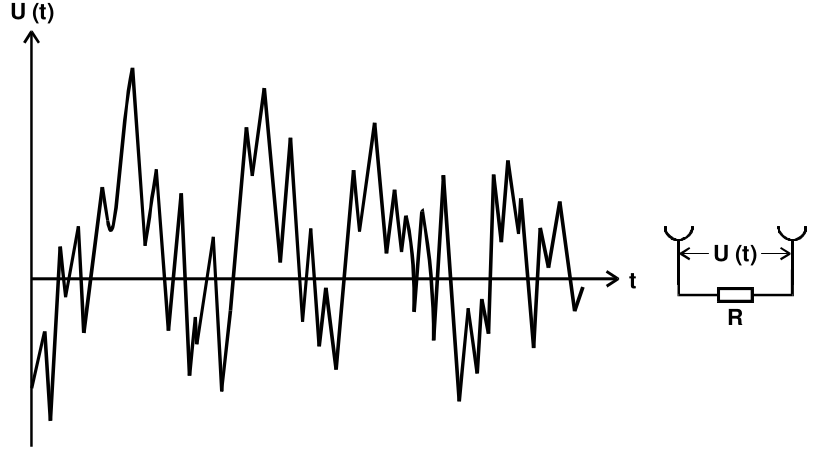
\includegraphics[scale=0.3]{bilder/rauschen.png}
  \caption{Typischer Spannungsverlauf an den Enden eines ohmschen Widerstands.}
\label{fig:rauschen}
\end{figure}
